\documentclass[twocolumn]{article}
\usepackage{graphicx}
%\usepackage{fancyhdr} 
%\usepackage{fancybox}
\usepackage{float}
\usepackage{listings}
\usepackage[colorlinks=true,urlcolor=black,linkcolor=black]{hyperref}
\usepackage[margin=1.0in]{geometry}
\usepackage{multicol}
\usepackage{type1cm}
\usepackage{lettrine}
%\pagestyle{fancy}

%redefines subsections with letters instesad of numbers
%\renewcommand{\thesubsection}{\thesection.\alph{subsection}}

% Center Image Command
\newcommand{\centerimage}[3]{
\begin{figure}[ht!]  
\begin{center} #1
\caption{#2}
\label{#3}
\end{center}
\end{figure}}

\newcommand{\centertable}[3]{
\begin{table}[ht!]  
\begin{center} #1
\caption{#2}
\label{#3}
\end{center}
\end{table}}

\title{\textbf{Branch Predictor and Branch Target Buffer} \\
ECE 486/586 Final Project }
\author{Eric Krause \hspace{1.4in} Bradon Kanyid\\
\url{ekrause@pdx.edu} \hspace{1in} \url{bradon@kanyid.org}}

\begin{document}
\twocolumn[
  \begin{@twocolumnfalse}
    \maketitle
    \begin{abstract}\textit{A branch predictor (modeled after the Alpha 21264 predictor) and a branch target buffer of our own design  were created and simulated.  These were used to predict the outcome and target of branches using 20 instruction traces from an ``unknown'' ISA, and achieved a rate of 13.059 target mispredicts per 1,000 branch instructions and a rate of  6.203 outcome mispredicts per 1,000 branch instructions.}
    \end{abstract}
  \end{@twocolumnfalse}
]
\textbf{Keywords:} Branch Prediction, Branch Target Buffer, Simulation,  ISA, 0xBEEFA55

\section{Background Information}
\lettrine{D}{uplication} of the tournament branch predictor used in the Alpha 21264 processor was the first objective of this project.  We then designed a corresponding branch target predictor.  The size budget for both parts of the project (Alpha predictor and branch target predictor) was 8,096 bytes.  The entire system was then tested against 20 instruction traces from an unknown ISA. \\\\
There were additional constraints as well: all table sizes had to be powers of 2, multiplying or dividing by numbers other than powers of two was not permitted, and tables with associativity $\ge$ 8 incurred a penalty equal to the size of the table.\\\\
Our branch predictor was modeled after the predictor described in R. E. Kessler's paper on the Alpha 21264 microprocessor.  Figure \ref{alpha} shows our implementation of the Alpha predictor.  One key difference between our implementation and Kessler's is that our predictor is only called on \textit{conditional branches}, not on all instructions.
\section{Branch Prediction}\centerimage{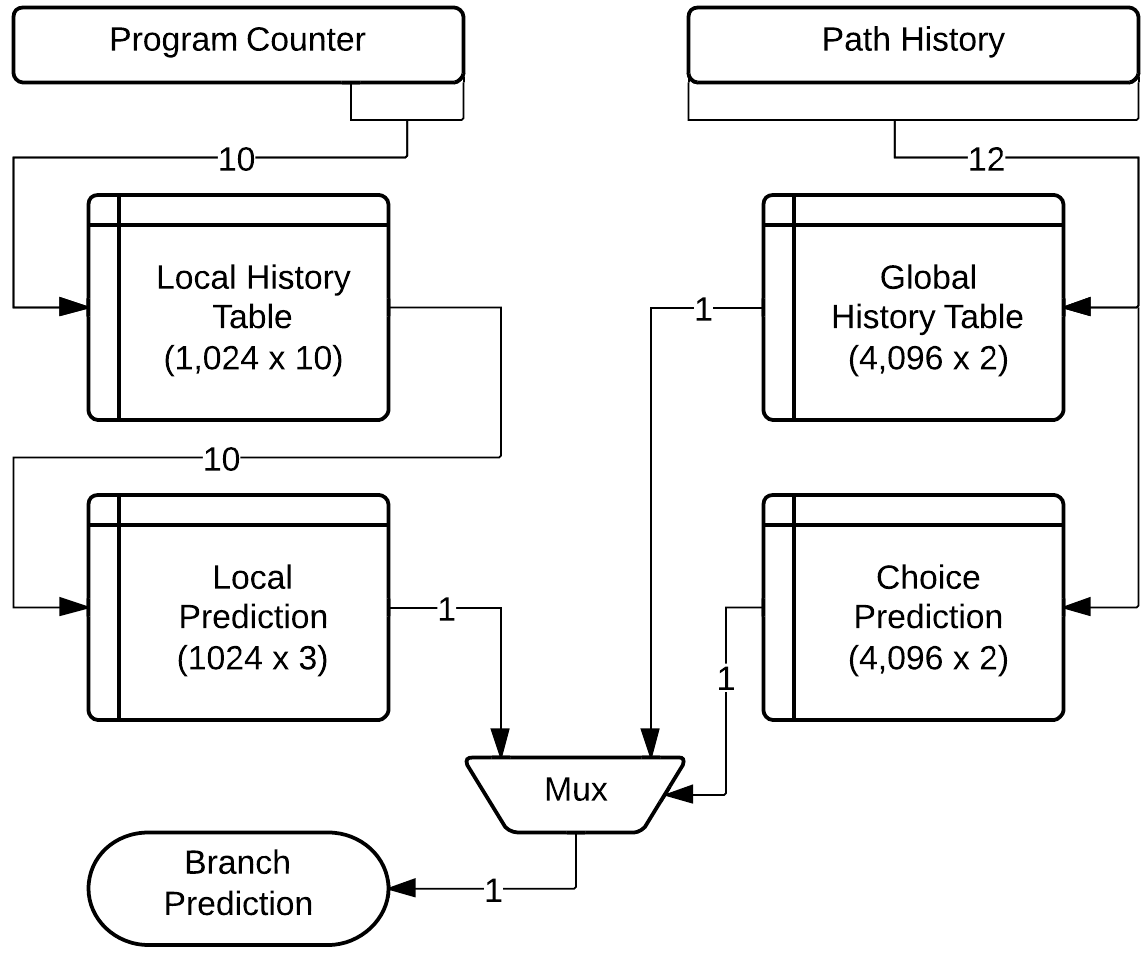
\includegraphics[width=\columnwidth]{img/alpha.png}}{Alpha Predictor}{alpha}\centerimage{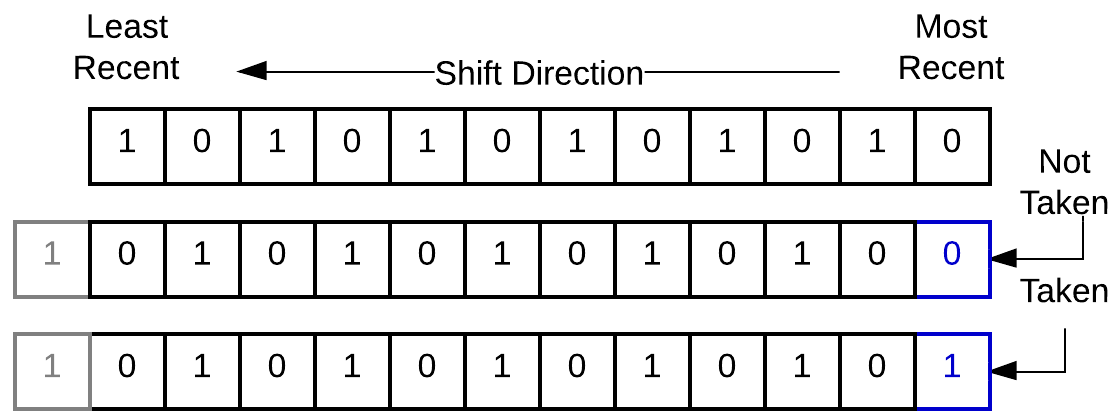
\includegraphics[width=\columnwidth]{img/phistory.png}}{Path History Shift Register}{phistory}
The Alpha predictor is a tournament predictor, meaning that it makes multiple predictions (based on the global and local histories) and then chooses between the prediction that has  been the most accurate, based on the path history.  The path history (illustrated in figure \ref{phistory}) is a shift register that maintains a history of the most recent 12 conditional branches by shifting in 1 or 0 (for taken or not taken branches respectively).\\\\
Path history is used as an index into the 4,096-entry choice prediction table, which maintains 2-bit saturating counters at each location which indicate whether--given the current path history--the local or global prediction has been more accurate.\\\\  
The global history table is also indexed using the path history, and consists of 4,096 2-bit saturating counters indicating whether--given the current global path history--the next branch is likely to be taken or not taken.\\\\
The local history table is indexed by the least significant 10 bits of the program counter.  Each entry in the local history table is a 10-bit path history for instructions (in our implementation, \textit{conditional branches}) with the same least significant 10 bits.  These local histories are used as indices into the local prediction table, which consists of 1,024 3-bit saturating counters indicating whether--given a local path history--the next branch is likely to be taken or not taken.\\\\
The strength of this design is that it can take advantage of branch patterns occurring within working sets of various sizes, with the local history being more useful with small working sets, and the global history being more useful for large working set.\\\\
A few implementation details were absent from Kessler's paper, so assumptions were made to create the most accurate predictor possible.  These fell into three categories:  Initialization values for the saturating counters and path history, under what conditions updates should occur, and how to handle unconditional branches (jumps).
\subsection{Initialization Values}
To start, everything was initialized to zero. This was to verify that our logic was working correctly. After verifying that things looked like they were working, we decided to see if tuning these parameters would have a major effect on our performance. Zeros would imply that our default state should be strongly not taken for both the local and global predictors, and strongly favoring the local predictor for the choice predictor.\\\\
For the initial states of each predictor, iteration through each value was possible in a reasonable amount of time. Doing so, we determined that locally weakly taken, globally weakly not taken, and choice weakly local gave best performance across all 20 benchmarks.
\subsection{Unconditional Branches}
The Alpha predictor on a hardware implementation would be used on every fetch, but in this simulation our predictor is only used for branches. Predictions are only neccessary for conditional branches, as unconditional branches are by definition always taken.
\subsection{Conditional Updates}
Our implementation of the Alpha branch predictor only updates the state of the predictor on conditional branches. To do otherwise would pollute the path history of the predictor, making it less effective. 
\section{Branch Target Prediction}
In a high-performance processor, simply predicting whether a branch is taken or not taken accurately is not enough to eliminate pipeline stalls.  If taken, the destination address of the branch must also be predicted so that instructions beginning at the target address can be speculatively executed. 
\subsection{Development History}
Our development process was much like a small weasel--somewhat iterative, yet dynamic and highly agile.  The space used for the branch predictor is 3,713 bytes (see table \ref{sizebudget} in Appendix A), meaning that any branch target predictor design had to fit in less than 4,382 bytes.
\subsubsection{Full Address Direct-Mapped Table}
Our initial design centered around using as much of the remaining 4,382 bytes as possible to create a single, large direct-mapped cache with 1,024 entries, each storing a single 32-bit address, for a total size of 4,096 bytes.  This approach was appealing because of its extremely simple implementation, and because it eliminated the need to store tags for any of the data.  Tags are not needed because there was no guarantee that the data returned was ``correct'' so any aliasing simply results in in a misprediction, which though not helpful is not catastrophic. \\\\
Upon completing this design, initial simulations using the first 4 trace files (FP-1, INT-1, MM-1, SERV-1) confirmed that aliasing was indeed a much larger problem than we had anticipated.
\subsubsection{Relative Offset Direct-Mapped Table}
In order to fit ``more cache'' into the available space, we redesigned the large cache from 3.1.1 to operate only on PC-relative branches, and only store the offset from the PC, which was only 24 bits.  This reduced the size of the table by 25\% to 3,072 bytes.  We had planned on using the additional 1024 bytes freed to create a smaller, wider cache that could store full 32-bit addresses that could not fit into the relative offset cache, however again, the amount of aliasing--even when considering only PC-relative branches--was far too high.\\\\
The smaller, 32-bit wide cache was never implemented because of the amount of aliasing that occurred with direct mapped caches, even when we increased the cache to be unrealistically large. 
\subsubsection{Victim Cache Missteps}
Later in our design process, we decided to use remaining space to implement a victim cache.  We apparently had not yet learned our lesson about direct-mapped caches, as the performance boost was minimal.  It quickly occurred to us upon seeing these results that a direct-mapped cache essentially defeats one of the main purposes of a victim cache: to handle cases of excessive aliasing and thrashing.\\\\
We then tested the other extreme, and experimented with a fully associative victim cache; although it would incur a penalty equal to its size, we thought the performance gain of a smaller, fully associative cache may outweigh the double size penalty.  Ultimately, the performance of a 30 entry fully associative cache was less than that of a 64-entry, 8 set x 8 way associative cache, and both took up the same amount of space. 
\subsection{Final Design}
Our final design abandoned all direct-mapped tables and focused on multi-way associativity to reduce aliasing.  Our final design consisted of a large 512-entry main cache (64 sets x 8 ways), a 64-entry victim cache (8 sets x 8 ways), and a 33-entry return address stack to handle returns. 
\subsubsection{Dynamic Objects}
Very soon after the direct-mapped cache approach was abandoned, the decision was made to design all objects with dynamic sizes, so that we could easily experiment with differently sized caches with no code changes.  Parameterized LRU and Cache objects greatly accelerated all testing and simulation efforts. 
\subsubsection{Main Cache}
The main cache was given highest priority in terms of space allocation.  The bold entries in table \ref{sizebydim} (Appendix A) indicate the largest possible configurations we could accommodate while staying under 4,382 bytes.  Gray values indicate configurations that are too large.  Table \ref{mispersize} (Appendix A) shows the relative performance  of select cache configurations.\\\\
Looking at the results from tables \ref{sizebydim} and \ref{mispersize}, the 64-set x 8-way configuration resulted in the best performance under the size constraints of our project.  We also took note of the fact that a 128-set x 4-way had the second best performance but used over 100 bytes less space.  If a problem had arisen that an additional 100 bytes could have solved, we would have made this change, but ultimately this was unnecessary. 
\subsubsection{Victim Cache}
The victim cache was given second highest priority in terms of space allocation.  Since the primary purpose of the victim cache is to accommodate aliasing spillover, we wanted the maximum associativity possible given our available space.   After deciding to use the 64x8 main cache, we had 542 bytes of space remaining.  We referred again to table \ref{sizebydim} and selected the 8-sets x 8-ways cache, with a size of 504 bytes.  
\subsubsection{Return Address Stack}
The main and victim caches cover the majority of cases, but one thing that cannot be predicted with the cache model are return addresses from calls. Returns are special cases of indirect branches, as the address to return to can be stored previously when a call instruction occurs. This relationship between calls and returns allows you to use a return address stack (RAS) to be able to return useful predictions for an indirect branch where this is almost impossible for other forms of indirect branches.\\\\ 
The RAS we implemented used a \texttt{deque}, as it had the right properties for our stack. Call addresses can be pushed onto the front of the \texttt{deque}, return addresses can be popped from the front of the \texttt{deque}, and if the stack becomes full, the oldest address can be popped from the back of the \texttt{deque}, keeping the stack within our size constraints.\\\\
The return address stack was much more flexible in terms of its size, since we were not limited to entry amounts that were powers of 2.  Hence, it was expanded to take up all of the remaining space, which yielded a 33-entry stack.
\section{Size Budget}
Our final design occupies 8,191 of the 8,192 available bytes. Table \ref{sizebudget} illustrates the exact breakdown of all elements in our project and their component parts, as well as the calculations to obtain these sizes.  We thought about encoding a snarky message in the leftover space, but all we could fit was \texttt{0xA5}.
\section{Results}
The results of running the 20 provided traces on our final design are shown in table \ref{results}:
\centertable{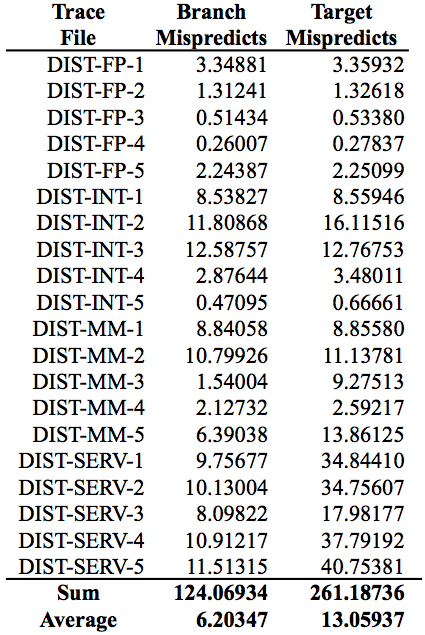
\includegraphics[width=2.5in]{img/results.png}}{Branch and target misprediction rates (per 1,000 branches)}{results}
\section{Conclusion}
For the most part, results of our simulations confirmed our initial assumptions, with a few key exceptions. Initially, we wanted to implement a direct-mapped cache, as not needing tags and LRU bits nearly doubled our possible table entries, but the sheer number of branches in each trace was simply overwhelming for any non-associative elements.  Also worth noting is how quickly the returns from a larger RAS diminish.  We considered resizing the caches to free up space for a larger RAS, but in our simulations increasing the number of stored return addresses--even to impossible extremes in the thousands resulted in very little improvement.\\\\
We would be interested to see the results of adding PC-relative displacement cache to our system.  Some calls and computed jumps will have 32-bit addresses, however nearly all conditional branches could be stored as offsets from the current PC, and since these account for the vast majority of branches in the traces provided, we could likely implement a much smaller cache for 32-bit addresses, and store all others as PC relative offsets, using a shared victim cache. We believe this model would offer even better performance than our approach, which unnecessarily uses 32-bit locations to store addresses that can very likely be stored in less than 32-bits.  However, considering we did not have time to explore this option, we are still very satisfied with our final results. 

\appendix
\onecolumn
\section{Tables}
\vspace{-.15in}\centertable{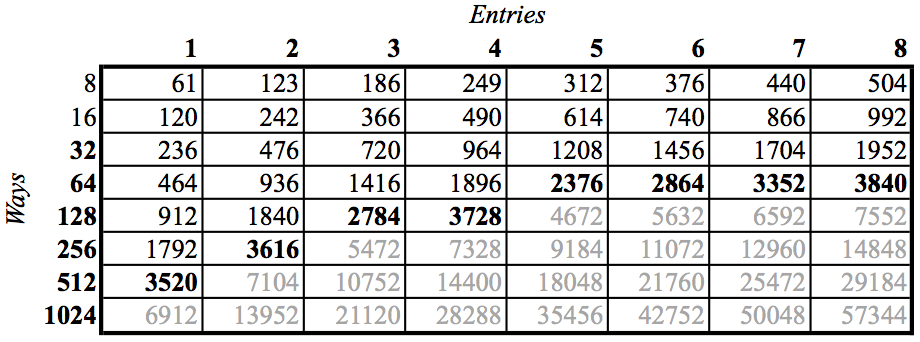
\includegraphics[width=5.25in]{img/sizebydim.png}}{Total space used (in bytes) for various cache dimensions}{sizebydim}
\vspace{-.35in}\centertable{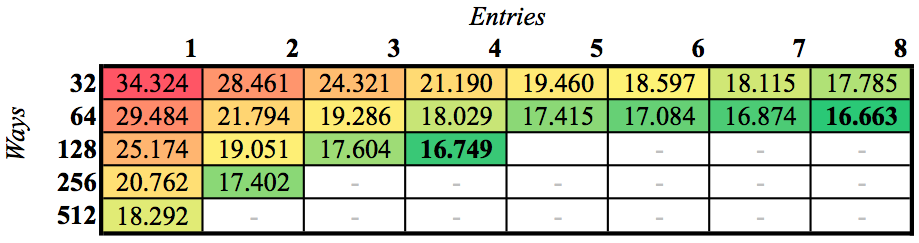
\includegraphics[width=5.25in]{img/mispersize.png}}{Target mispredictions/1000 instructions (Average of FP-1, INT-1, MM-1, and SERV-1 traces)}{mispersize}
\centertable{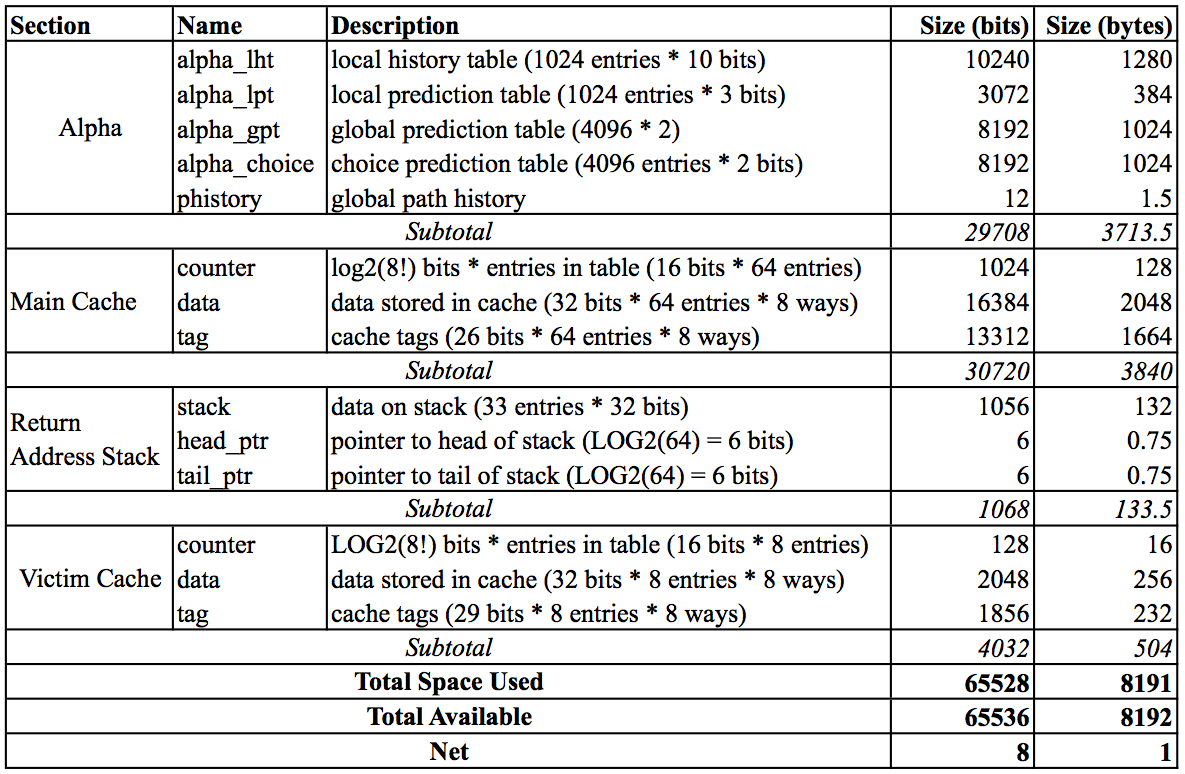
\includegraphics[width=\columnwidth]{img/sizebudget.png}}{Total size of all project elements}{sizebudget}
\section{Source Code}

\subsection*{Header}
\lstinputlisting[language=C++, showstringspaces=false, numbers=left, numberstyle=\tiny, numberblanklines=true]{../predictor.h}

\newpage
\subsection*{Implementation}
\lstinputlisting[language=C++, showstringspaces=false, numbers=left, numberstyle=\tiny, numberblanklines=true]{../predictor.cc}
\end{document}
